\section{Riggin' Captain Kangaroo}

\margininbox{Captain Kangaroo}{
     \begin{itemize}
    \item Richard Venn
    \item Tharatorn Supasiti
    \end{itemize}}{\explo}

First trip was with Thara. Tet had already rigged down \passage{Pico} (re-bolting
it in the process), so we set off for that familiar window with a
bolting hammer, a hundred metres of rope and a couple of cinnamon malt
loaves. Had the same trouble finding Tet's single bolt as I'd had in
2005. However, instead of bottling it, I placed two new spitz, this time
within sensible reach for easy rigging. A hundred metres of rope got us
to \passage{Traverse Chamber}, cursing and kicking the heavy bag all the way
through \passage{Scrotty}.

\margininbox{Captain Kangaroo}{
     \begin{itemize}
    \item Richard Venn
    \item Sandeep Mavadia
    \end{itemize}}{\explo}

Sandeep was the next victim, this time we set off with a hundred and
fifty metres of rope. We rigged down to \passage{Olympic Rift}, stopping on the
way to chisel open an awkward squeeze. We left thirty metres of rope in
a tacklesack at the start of \passage{Olympic Rift} and did some re-bolting on the
last two pitches. Also left three hangers and maillons, ten spits \&
cones, two karabiners, a chisel and two slings. At this stage the
squeeze and huge black space the other side at the end of \passage{Olympic rift}
seemed like the best lead in \passage{Captain Kangaroo}.

A bounce to \passage{Pico} with James gave me the chance to do some more work on
the entrance to \passage{Captain Kangaroo}. I put in a tensioned traverse which
removed the `traditional' rub-point at the start of the take off.

\name{Richard Venn}


\section{Pushin' Captain Kangaroo}

\margininbox{Captain Kangaroo}{
     \begin{itemize}
    \item Richard Venn
    \item Ben Banfield
    \end{itemize}}{\explo}

I had hoped that keen cavers would rush into \passage{Captain Kangaroo} to push
the more shallow lead off \passage{Traverse Chamber}, leaving me to go and smash
open \passage{Olympic Rift} to fame and great glory in whatever gaping chasm lay
beyond the terminal squeeze. Unfortunately, Vom-Brown \sidenote {Tom Brown} and the Deep \sidenote {Sandeep Mavadia}
turned back near \passage{Bonus Chamber}, with `visions of hell' muttered back at
the bivvi from the first sign of mild scrotty-ness.

I collared young Ben in the bivvi over a generous swig or two of
rum-spiked tea and we hatched a plan to crawl along a tight rift that
I'd looked down with Jarv in 2005, but been unable to survey due to lack
of tape. With survey pencils and instruments in tow, we slipped through
the cave to the pushing front and stripped off SRT kits to pass more
easily through the rift. This was somewhat tighter than I'd remembered
and shredded my PVC oversuit.

\bignote{We pushed as far as we dared survey}, breaking out right at end into a
large double chamber with several leads coming off. The most obvious of
these was a climb down into what looked like walking passage.

Returning a few days later with Izzy\sidenote {Iztok Možir} from Tolmin, with a bag of rope and
bolting kit, we pushed the passage another fifty metres or so. Some
gardening of large rocks was required to pass a short section of rift
but we were mostly in big passage, clambering down rather sharply over a
series of climbs.

\begin{marginfigure}
\frame{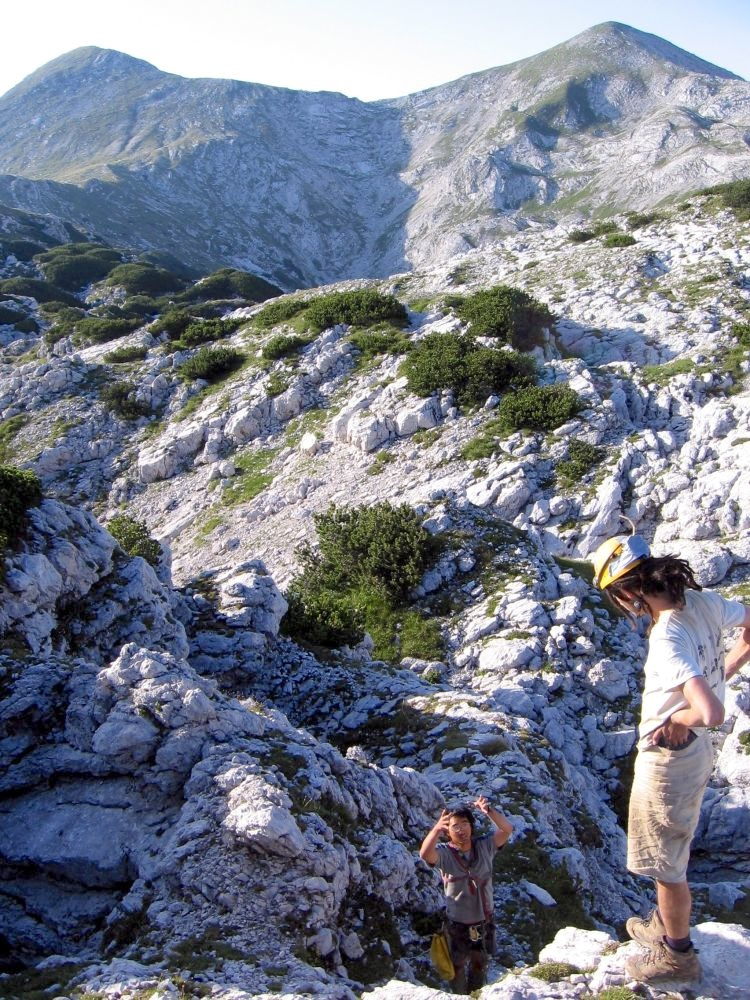
\includegraphics[width = \textwidth]{2007/kangaroo/jarvist frost - m1 - rik and thara after bolting--orig.jpg}}
\caption{Rik and Thara after their bolting trip, standing beside \passage{M1} \pic{Jarvist Frost}}
\end{marginfigure}

Eventually we reached a point where a big passage closed up to about one
or two metres of very tight rift with a big (approx. two second) drop on
the other side. This was passable but looked more than a little
unpleasant without some serious work with a chisel.

We looked around the chamber a little more before discovering a tight
sharp crawl which dog-legged before coming out in beautiful white rock
at the top of a twenty metre pitch. Izzy belayed my full weight from
within the crawl while I put in the two bolts. This allowed us to
descend to the bottom of the pitch with a few metres of rope to spare.
This is possibly not the same pitch we were throwing rocks down through
the tight rift but obviously very close!

As we dropped the pitch there were windows on both sides looking like
they came from either other pitches or more rift-like development as
well as two leads at the bottom. These were a small \passage{Captain Kangaroo}-esque rift and ten or twenty metres more of the pitch. We left
\textasciitilde{}10 m of rope, but took the tacklesack out.

This was a very exciting new section of passage. We named the contents
of our push ``\passage{Kill em All}'' after the first Metallica album. Upon
inspection of our survey data, it became clear that we were exceedingly
close to passage below \passage{Silos}/\passage{Godzilla} in \passage{M2} (less than thirty
metres at closest approach).

Unfortunately, a month on Migovec was starting to catch up with me and
though I wanted another trip in \passage{Gardeners' World} to push \passage{Olympic rift}, I
was completely exhausted with very sore knees. The leads we left in
\passage{Captain Kangaroo} this year will be far too tantalising to sideline in favour of
surface work in 2008. The prospect of a connection with the system seems
very likely and next year we're already planning a return to \passage{M2}
to resurvey (our current data comes from a 1970s survey carried out with
a home-built clinometer!) and to exhaust the deep leads.

\name{Richard Venn}

\begin{pagefigure}
\checkoddpage \ifoddpage \forcerectofloat \else \forceversofloat \fi
   \centering
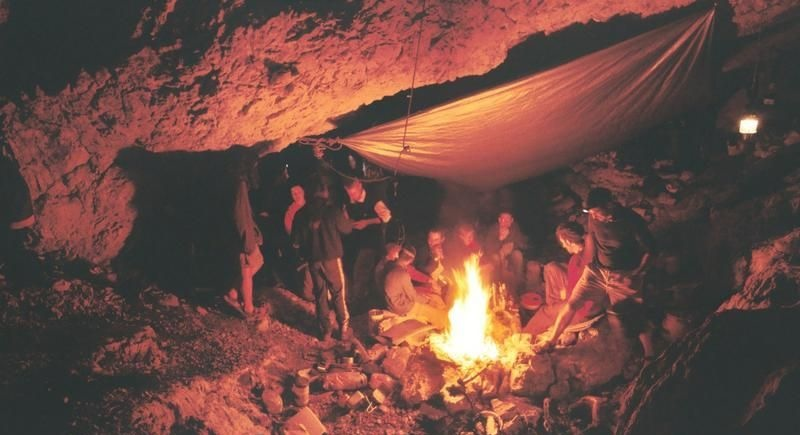
\includegraphics[width = 0.6\textwidth]{2007/kangaroo/jarvist frost gr1 film2 -031_28.jpg}
\caption{A typical evening in the bivi around the fire \pic{Jarvist Frost}}
\end{pagefigure}

\begin{pagesurvey}
\centering
\frame{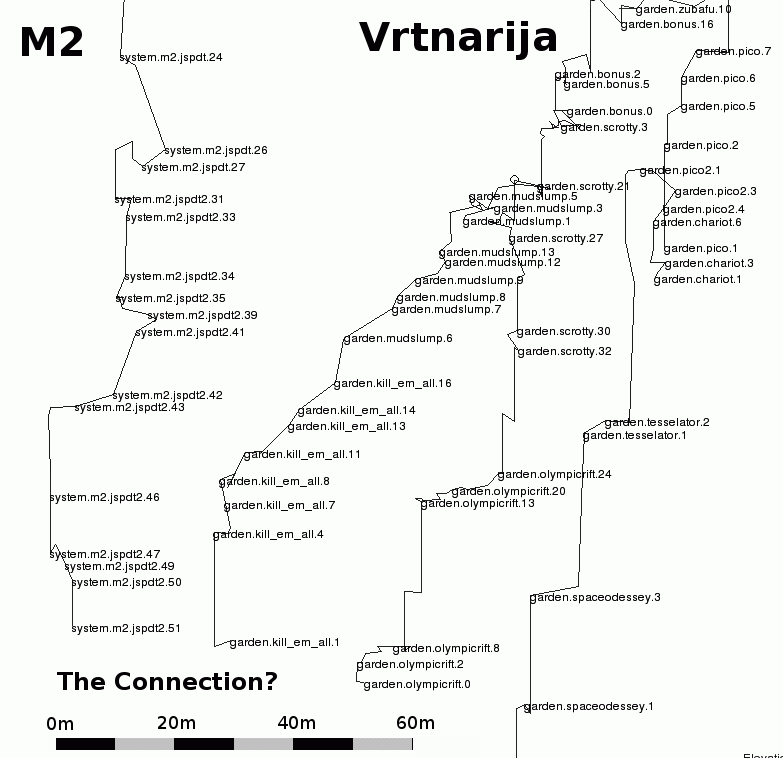
\includegraphics[width=\textwidth]{2007/kangaroo/survex - 2007 data - m2 vrtnarija closest approach--orig.png}}
\caption[M2 Vrtnarija Closest Approach]{Survey data of the closest approach between \passage{M2} and \passage{Gardeners' World}.}
\label{plan 2013}
\end{pagesurvey}
